\chapter{Incorporating Clustering Information into Peak Alignment}
\label{c:matching}

% \textbf{Summary.} In this chapter, we introduce mixture modelling to cluster related peaks by their retention time. The clustering information is then used to modify the similarity matrix used in a direct-matching method, allowing for peak across correspondent groups to be brought closer during matching. Our validation against benchmark datasets show that the proposed method ...

\section{Introduction}

In liquid chromatography measurements, peaks can experience non-linear shift in retention time (RT) values across runs \cite{Podwojski2009}. RT variation could be due to instrument-specific factors (the condition of the chromatographic column itself. including flow rate variations, gradient slope and temperature \cite{Christin2008}) or experiment-specific factors (e.g. instrument malfunctions or columns that need be replaced mid-experiment). In direct matching, several potential matches may be present for a peak from one run to another, but because the elution order of correspondent peaks may swap across runs \cite{Smith2013}, the candidate peaks nearest in distance are not necessarily the correct match.

As described in Section~\ref{sub:grouping-background}, ionization product (IP) peaks are the set of chemically-related peaks produced from the mass spectrometry measurement of a single compound, such as a peptide fragment (in the case of proteomics) or a metabolite (in metabolomics). Examples of IP peaks are isotope peaks, multiple adduct and deduct peaks, and fragment peaks. IP peaks of the same compound have similar chromatographic peak shapes as they co-elute from the column. Such information could potentially be used to improve matching since a group of IP peaks in one run should generally be aligned to another group of IP peaks in the other run. In the direct-matching approach (discussed in Section~\ref{sub:alignment-tools}), correspondent peaks from one run to another are directly matched to each other without first correcting for RT drift (instead the assumption on RT noise is built into the distance/similarity function used for matching). A direct matching method can take this structural information of IP peaks into account in order to improve alignment, however none of the direct matching methods discussed in Section~\ref{sub:alignment-tools} exploit this information.

In this chapter, we propose clustering IP peaks that share similar RT values together. This clustering information is used to modify the similarity score matrix used for matching to bring groups of IP peaks that should be matched closer, with the key assumption that groups of co-eluting peaks corresponding to the same metabolite are generally preserved across runs. This idea is illustrated in Figure~\ref{fig:computingweight} and further introduced in Sections~\ref{sub:direct-matching} and ~\ref{sub:incorporating-grouping}.  

\begin{figure*}[!htbp]
\centering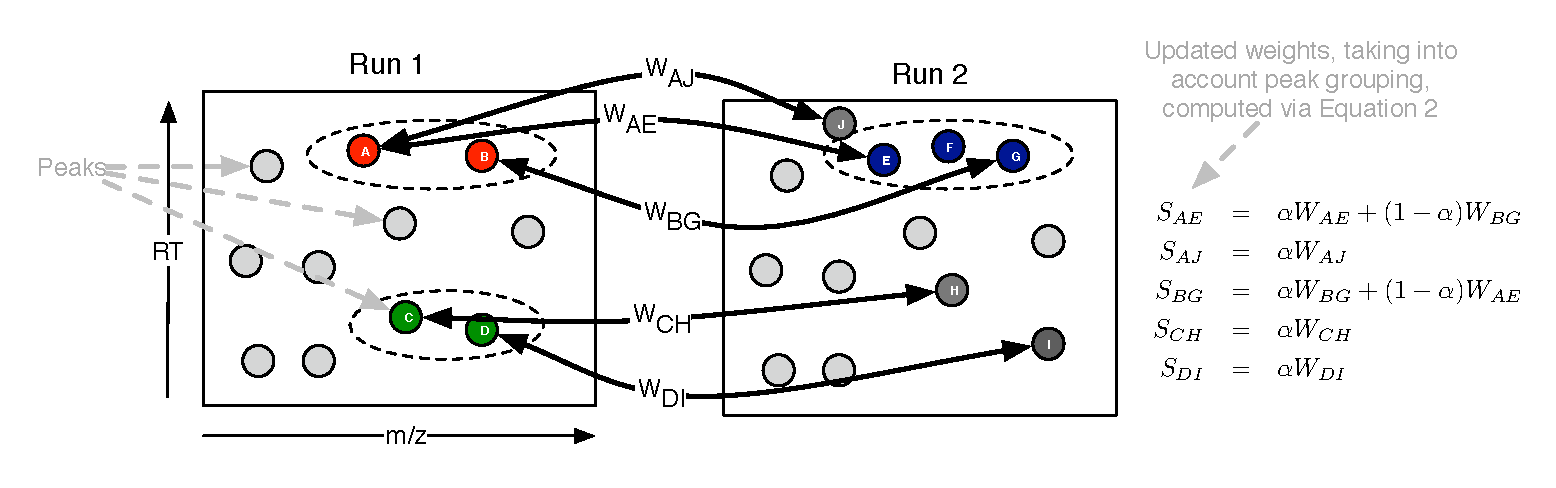
\includegraphics[width=1\linewidth]{04-matching/figures/figure_1.eps}
\centering\caption[Illustrative example of the incorporation of grouping information into the similarity score.]{\label{fig:computingweight} Illustrative example of the incorporation of grouping information into the similarity score. Each node in the figure is a peak feature, and dotted ovals represent groups of IP peaks, e.g. isotopes, fragments, etc. Initially weights (e.g. $W_{AE}$) are computed for pairs of peaks (one from each run) with m/z and RT within pre-defined thresholds. These weights are converted into an overall score by incorporating grouping information. For example, peak pairs $(A,E)$ and $(B,G)$ are both within the threshold. Because $A$ and $B$ are in the same group, and $E$ and $G$ are in the same group, the weights between pairs $(A,E)$ and $(B,G)$ are upweighted. Peak $J$ is not related to any peaks that could be matched with $A$'s IP peaks and the similarity between $A$ and $J$ is therefore downweighted (because $\alpha\leq 1$). The same applies to similarities between pairs $(C,H)$ and $(D,I)$.}
\end{figure*}

As shown in Figure~\ref{fig:computingweight}, initial weights are computed between pairs of peaks in the two runs that are within m/z and RT tolerances (e.g. $W_{AE}$ and $W_{AJ}$). When related peak information is added, the similarity between peaks $A$ and $E$ is increased due to peak $A$ being related to another peak ($B$) that is similar to a peak ($G$) related to $E$. On the other hand, the similarity between $A$ and $J$ is not increased as $J$ does not have any IP peaks that could potentially be matched to peaks related to $A$. In other words, we are proposing using the structural dependencies present between peaks in each run to modify the similarity scores and improve alignment performance: the more peaks related to $A$ that could be matched to peaks related to $E$, the more likely it becomes that $A$ should be matched to $E$.

\section{Related Work}

Direct matching is introduced in Section~\ref{sub:alignment-tools}, while the grouping of IP peaks is introduced in Section~\ref{sub:grouping-background}. 

\subsection*{Statement of Original Work}

The work from this chapter has been published in \textit{Bioinformatics} \cite{wandy2015incorporating}. The author proposed and implemented the idea of incorporating clustering information into a direct-matching alignment method. The author also performed the evaluation of performance of the proposed approach against the baseline methods. 

\section{A Direct Matching Method That Incorporates Clustering Information\label{sub:direct-matching}}

Our proposed alignment method combines a novel similarity score with maximum weighted bipartite matching. This results in pairwise alignments which can be, if desired, extended to multiple alignments with hierarchical merging strategy. In such merging strategies, having an accurate initial pairwise alignments is important because of its influence on the final multiple alignment results. Here, we describe a direct matching approach to performing alignment of peaks across two LC-MS runs. 

A peak feature refers to a tuple of $(m/z,RT)$ produced as output after the initial peak detection stage of LC-MS data. Here, m/z is the mass-to-charge value and RT the retention time value of a peak feature. Suppose we wish to align run A containing $N_A$ peaks with run B containing $N_B$ peaks.  Alignment between two runs can be represented as a matching problem on a bipartite graph $G$, where nodes in the graph are the features, edges are the potential correspondence between features and the weights on the edges are the similarity scores (entries in $S$) between features. In SIMA \cite{Voss2011a}, the Gale-Shapley algorithm \cite{Gusfield1989} is used to find a stable matching in $G$. A matching is stable if there are no two features in different runs that would prefer to be matched to each other than to their currently matched partners. Since the stable matching is computed based on ranked preference, valuable information could be discarded as distances between features are converted to ranks. As such, we prefer to use a method that maximises the total sum of similarity scores of matched features (maximum weighted matching).

The benefit of maximum weighted bipartite matching in solving the peak correspondence problem has been studied in \cite{Wang2013} in their LWBMatch tool. LWBMatch shows that such matching method, coupled to a local regression method, is able to align runs having large and systematic drifts in RT values. The well-known Hungarian algorithm \cite{Kuhn1955} attributed to Kuhn and Munkres is used in LWBMatch to solve this problem. The time complexity of the Hungarian algorithm is $O(n^{3})$, where $n$ is the number of peaks in the larger set. While the Hungarian algorithm's implementation can be improved to $O(n^{2}log\, n)$ by using Fibonacci heaps for the shortest path computation, the polynomial time complexity required in this scheme is often too slow to be practical for alignments of the large number of runs produced in large-scale untargeted LC-MS studies. Consequently, we compute an approximation of the maximum weighted matching using a simple greedy algorithm that runs in $O(m\, log\, n)$ time, where $n$ and $m$ denote the number of vertices and edges in the bipartite graph $G$ to be solved. The greedy algorithm is straightforward to describe: pick the heaviest edge $e$ in $G$, where $e$ represents a potential match between nodes (features). Add $e$ to the matching solution $M$ and remove all other edges adjacent to $e$ from $G$. Repeat until all edges in $G$ have been exhausted. This simple greedy algorithm is known to provide a lower bound of at least 1/2 of the maximum weight in the matching \cite{Maximum2011}. From the direct matching of peaks across two runs, we obtain a list of aligned peaksets, defined as the sets of correspondent peaks that have been matched across runs. In the case of two runs, an aligned peakset has a size of at most 2.

\subsection{Feature Similarity}

To define a similarity measure between peaks, we follow SIMA \cite{Voss2011a} in using the Mahalanobis distance between two peaks $\boldsymbol{p}_{i}\in A$, $\boldsymbol{p}_{j}\in B$ where each peak is a vector of its m/z and RT values $\boldsymbol{p}_{i}=[m_{i},t_{i}]^\trans$ and $\boldsymbol{p}_{j}=[m_{j},t_{j}]^\trans$. The distance is given as: 
\[
D(\boldsymbol{p}_{i},\boldsymbol{p}_{j})=\sqrt{(\boldsymbol{p}_{i}-\boldsymbol{p}_{j})^{\trans}\boldsymbol{\Sigma}^{-1}(\boldsymbol{p}_{i}-\boldsymbol{p}_{j})},
\]
where the covariance matrix $\boldsymbol{\Sigma}$ is a diagonal matrix of mass-to-charge tolerance $\sigma^2_{m}$ and retention time tolerance $\sigma^2_{t}$. The diagonal covariance matrix $\boldsymbol{\Sigma}$ assumes independence between the $\sigma^2_{m}$ and $\sigma^2_{t}$ components since measurement error in m/z is independent of RT. To reduce the computational burden, entries in $\boldsymbol{D}$ are only computed when the peaks' m/z and RT values are within $\sigma_{m}$ and $\sigma_{t}$. We now define the similarity score between two peaks as one minus their normalised distance:
\begin{equation}
W(\boldsymbol{p}_{i},\boldsymbol{p}_{j})=1-\frac{D(\boldsymbol{p}_{i},\boldsymbol{p}_{j})}{D_{max}},
\end{equation}
where $D_{max}$ is the maximum computed distance between peaks in the two runs being aligned. Collectively, we call the $N_A\times N_B$ matrix of similarity scores between all peaks in run A and B to be $\boldsymbol{W}$. 

\subsection{Combining Related Peak Information\label{sub:incorporating-grouping}}

The similarity score matrix $\mathbf{W}$ can now be combined with related peak information to obtain a final score, $\mathbf{S}$:
\begin{equation}\label{eq:combining-eq}
\boldsymbol{S}=\alpha \boldsymbol{W}+(1-\alpha)\boldsymbol{L}
\end{equation}
where $\boldsymbol{L}$ is the cluster similarity score between the two peaks in a single run (described below), and $\alpha$ ($0\leq\alpha\leq1$) is a parameter controlling the relative influence of the two components. To compute $\boldsymbol{L}$, we require related peak groupings from the two runs being aligned. This takes the form of an $N_A\times N_A$ matrix $\mathbf{C}^A$ for run A and an $N_B\times N_B$ matrix $\mathbf{C}^B$ for run B. Entries in $\boldsymbol{C}^A$ and $\boldsymbol{C}^B$ can be either binary (0, 1) or probability values, depending on the peak grouping algorithm used. For example, if a greedy clustering approach is applied to the features in run A, the $ij$-th element of $\mathbf{C}^A$ will be either 1 or 0, depending on whether the $i$-th and $j$-th features (peaks) in A are clustered together (1) or not (0). Note that in the following, we define the diagonal components of both matrices to be zero to avoid double counting. We then compute $\mathbf{L}$ as follows:
\begin{equation}\label{eq:L-multiply}
\boldsymbol{L}=\boldsymbol{C}^A \cdot \boldsymbol{W} \cdot \boldsymbol{C}^B.
\end{equation}
The resulting matrix gives cluster similarity scores such that each element $L_{ij}$ of $\boldsymbol{L}$ is the sum of weight from peaks in the same cluster as $i$ in run $A$ to peaks in the same cluster as $j$ in run $B$. This allows us to use the matrix $\boldsymbol{L}$ to upweight the similarity scores between peaks in the same cluster in one run that also have more potential matches to peaks in the same cluster in the other run of the matching. Computation of Equation~\ref{eq:L-multiply} is illustrated in Figure \ref{fig:computingweight}. The ratio parameter $\alpha$ controls how much clustering information we bring into the overall similarity score matrix $\boldsymbol{S}$, with its value bounded in $0\leq\alpha\leq1$. Setting $\alpha=1$ results in a matching that uses only information from $\boldsymbol{W}$, the similarity score matrix. Setting $\alpha=0$ means that the matching is performed based only on the cluster similarity score $\boldsymbol{L}$. From our experience, a reasonable range of values for $\alpha$ lies between $0.2$ to $0.4$.

Our proposed approach is independent of the method used to group IP peaks in each run. For comparison, we call our method that does not use the cluster similarity score ($\alpha=1$) to be \ac{MW}. We then demonstrate the performance improvement from incorporating IP peaks information using two different clustering algorithms: a greedy RT clustering approach (described in Section~\ref{sub:rt-clustering-greedy}) and a statistical mixture model (Section~\ref{sub:rt-clustering-mixture}). The combination of matching with the greedy clustering is called MWG, while the alternative approach that uses the probabilities coming from the mixture model is called MWM.

\subsection{Greedy Clustering of IP peaks\label{sub:rt-clustering-greedy}}

In the greedy clustering method, the most intense peak in the dataset is selected and clustered with other candidate peaks inside a retention time window $g_{tol}$. The next most intense peak that has not already been clustered is processed, and the grouping process is repeated until all peaks are exhausted. If chromatographic peak shapes information is available (such as for the Metabolomic dataset used in section \ref{sub:Metabolomic-glycomic-experiments}), the Pearson correlation coefficient between the chromatographic peak signals of the most intense peak and the candidate peaks are computed. Only candidate peaks with Pearson correlation values greater than some threshold $c$ are accepted into the newly-formed cluster. This greedy clustering process results in binary grouping matrices $\mathbf{C}^A$ and $\mathbf{C}^B$ that can be used in eq. \ref{eq:L-multiply}.

\subsection{Mixture Model Clustering of IP peaks\label{sub:rt-clustering-mixture}}

We can also group IP peaks together by their RT values using a mixture model. Our observation consists of a vector of $N$ observed peak's RT values $\mathbf{y}=(y_{1},y_{2},...,y_{n})$, and our aim is to partition each set of peaks into $K$ groups of IP peaks (clusters) by their RT values. We used a Gaussian mixture model with Dirichlet Process prior (described further in Section~\ref{background-dp-clustering}) to model the data. A peak is indexed by the variable $n=1,...,N$ and a cluster indexed by the variable $k=1,...,K$. Each Gaussian mixture component has some mean $\mu_{k}$ are assumed to have a fixed precision (inverse variance) $\delta$, corresponding to the fixed retention time tolerance for each group of IP peaks. Let the indicator $\boldsymbol{z}_{nk}=1$ denotes the assignment of peak $n$ to RT cluster $k$. Then: 
\begin{eqnarray}
\boldsymbol{\pi}|\alpha & \sim & GEM(\gamma)\\
\boldsymbol{z}_{nk}=1|\boldsymbol{\pi}_{k} & \sim & \boldsymbol{\pi}_{k}\\
\mu_{k}|\mu_{0},\tau_{0} & \sim & \mathcal{N}(\mu_{k}|\mu_{0},\tau_{0}^{-1})\\
y_{n}|\boldsymbol{z}_{nk}=1,\mu_{k} & \sim & \mathcal{N}(\mu_{k},\delta^{-1})
\end{eqnarray}
where $\boldsymbol{\pi}$ is the mixing proportions, distributed according to the GEM (Griffiths, Engen and McCloskey) distribution. The GEM distribution over $\boldsymbol{\pi}$ is parameterised by the concentration parameter $\gamma$ and is described through the stick-breaking construction:
\begin{eqnarray}
\beta_{k} & \sim & Beta(1,\gamma)\\
\boldsymbol{\pi}_{k} & = & \beta_{k}\prod_{l=1}^{k-1}(1-\beta_{l})
\end{eqnarray}
The mixture component mean $\mu_{k}$ is drawn from a base Gaussian distribution with mean $\mu_{0}$ and precision $\tau_{0}$. We set $\mu_{0}$ to the mean of the observed data, while $\tau_{0}$ is set to a broad value of 5E-3. Analytical inference is not tractable here, so we use the Gibbs sampling scheme for inference. To do this, we need the conditional probability of $p(\boldsymbol{z}_{nk}=1,...)$ of peak $n$ to be in an existing cluster $k$ (or $k^{*}$ if a new cluster is to be created), given any other parameters in the model. This conditional probability is given by:
\begin{equation}
P(\boldsymbol{z}_{nk}=1|\mathbf{y}_{n},\ldots)\propto\begin{cases}
\begin{array}{c}
c_{k}\cdot p(\mathbf{y}_{n}|\boldsymbol{z}_{nk}=1,...)\\
\gamma\cdot p(\mathbf{y}_{n}|\boldsymbol{z}_{nk^{*}}=1,...)
\end{array}\end{cases}\label{eq:table_likelihood}
\end{equation}
where $c_{k}$ is the current number of members (peaks) in an existing cluster $k$. $p(\mathbf{y}_{n}|\boldsymbol{z}_{nk}=1,...)$ is the likelihood of peak $\mathbf{y}_{n}$ in an existing cluster $k$. We can marginalise over all mixture components and get: 
\begin{eqnarray}
p(\mathbf{y}_{n}|\boldsymbol{z}_{nk}=1...) & = & \mathcal{N}(\mathbf{y}_{n}|\mu_{k},\lambda_{k}^{-1})\label{eq:15}
\end{eqnarray}
where $\lambda_{k}=((\tau_{0}+\sigma c_{k})^{-1}+\delta^{-1})^{-1}$ and $\mu_{k}=\frac{1}{\lambda_{k}}\left[(\mu_{0}\tau_{0})+(\delta\sum_{n}\mathbf{y}_{n\in k})\right]$. Here, $\mathbf{y}_{n\in k}$ denotes the RT values of any peak $n$ currently assigned to cluster $k$, and $c_{k}$ the count of such peaks. The conditional probability of peak $n$ to be in a new cluster
$k^{*}$ is:
\begin{eqnarray}
p(\mathbf{y}_{n}|\boldsymbol{z}_{nk^{*}}=1...) & = & \mathcal{N}(\mathbf{y}_{n}|\mu_{0},\lambda_{k^{*}}^{-1})\label{eq:15-1}
\end{eqnarray}
where $\lambda_{k^{*}}=(\tau_{0}^{-1}+\sigma^{-1})^{-1}$.
In a step of the Gibbs sampling procedure, we perform the assignment of peak $n$ to cluster $k$, creating new cluster $k^{*}$ if necessary. Using the posterior summaries across all samples drawn $S^{*}=\frac{1}{R}\sum_{r=1}^{R}s{}_{r}$, where $s{}_{r}$ is the $r$-th posterior sample collected after a suitable burn-in period and $R$ is the total number of samples taken (excluding burn-in samples), we can obtain the marginal posterior of the probability of two features (peaks) to be in the same cluster $k$ averaged across all samples. These probabilities comprise the elements of $\mathbf{C}^A$ and $\mathbf{C}^B$ (i.e.\ the $ij$-th element of $\mathbf{C}^A$ is the proportion of samples from run A in which peaks $i$ and $j$ were in the same cluster), which can be used in eq. \ref{eq:L-multiply}.

\section{Evaluation Study\label{sub:evaluation-study}}

Performance evaluation of alignment methods is difficult due to the lack of gold standard and evaluation criteria for benchmarking \cite{Castillo2011,Smith2013a}. Relatively few works, such as \cite{Lange2008}, exists that provide a comprehensive ground truth for evaluation. In fact, despite the numerous alignment methods that exist, most methods remain unevaluated, evaluated against a small number of alternatives or evaluated based on highly subjective criteria \cite{Smith2013}. In particular, evaluation of alignment quality through manual visual inspection of superimposed profile images and some selected chromatograms is problematic and is not a systematic approach towards performance evaluation. While straightforward, the visual inspection of alignment quality is tedious and do not work for evaluation of a large number of aligned peaksets produced by the alignment of a large number of samples. It is also often subjective and might suffer from dissimilar interpretations across different experiments and datasets. 

In this chapter, the performance of the proposed methods and other benchmark methods is evaluated using precision and recall on LC-MS datasets from proteomic, metabolomic and glycomic experiments. The proteomic datasets are obtained from \cite{Lange2008} while the glycomic dataset comes from \cite{Tsai2013a}. These datasets provide the ground truth for alignment and have used to benchmark alignment performance in other evaluation studies \cite{Lange2008, Pluskal2010, Ballardini2011, Voss2011a, Tsai2013a}. Additionally, we also introduce a metabolomic dataset generated from the standard runs used for the calibration of chromatographic columns \cite{Creek2011}. The runs were produced from different LC-MS analyses separated by weeks, representing a challenging alignment scenario. 

Many direct matching methods work in a pairwise fashion and produce an overall results via some merging strategies of intermediate results. Pairwise performance therefore limits overall performance, and as such, in this chapter, we focus on evaluation using only pairs of runs. Some (P2, metabolomic and glycomic) of the datasets selected for evaluation in our experiments have more than 2 runs, so we select only 2 runs each to form a training and testing set. The procedure for doing so is described in the respective following sections for each dataset.

\subsection{Proteomic Datasets\label{sub:proteomic-dataset}}

\cite{Lange2008} introduces two benchmark LC-MS proteomic sets (P1, P2) constructed to evaluate the ability of alignment tools in dealing with large retention time drifts. Both the P1 and P2 datasets were analysed using an automated LC-LC/MS-MS platform. Each dataset comes in multiple chromatography salt-step fractions, obtained by bumping the salt level at every 10 minutes interval during chromatographic separation. P1 was produced from \textrm{\textit{E. coli}} samples digested by trypsin, and comes in 2 runs for each fraction. P2 was obtained from \textrm{\textit{M. smegatis}} protein extracts, similarly digested by trypsin, and contains 3 runs for each fraction. P2 was constructed to be a greater challenge to align with runs separated by weeks. Alignment ground truth is established in \cite{Lange2008} by means of peptides that can be reliably identified during the identification stage. Only identification annotations with SEQUEST Xcorr score \textgreater 1.2 is included. Annotations are then filtered by their retention times and matched across runs. 

For the proteomic datasets, each fraction in P1 has two runs used for alignment, while each fraction in P2 has three runs (we use only the first two to establish pairwise alignments). Tables \ref{tab:No.-of-features-P1} shows the number of features for each run of the P1 and P2 datasets used for evaluations. Both P1 and P2 represent challenging alignment cases, with large deviations in RT values across runs. This is especially true for P2 with LC-MS runs separated by weeks and large differences in the number of features per run. Further details on the nature of the datasets can be found in \cite{Lange2008}. 

\begin{table}[!htbp]
\noindent \begin{centering}
\begin{tabular}{|c|c|c|c|}
\hline 
Fraction & \# runs & \# features per run (P1) & \# features per run (P2)\tabularnewline
\hline 
\hline 
\multirow{2}{*}{000} & \multirow{2}{*}{2} & 5824 & 5054\tabularnewline
\cline{3-4} 
 &  & 4782 & 5100\tabularnewline
\hline 
\multirow{2}{*}{020} & \multirow{2}{*}{2} & 1114 & 3271\tabularnewline
\cline{3-4} 
 &  & 1021 & 529\tabularnewline
\hline 
\multirow{2}{*}{040} & \multirow{2}{*}{2} & 1230 & 1483\tabularnewline
\cline{3-4} 
 &  & 958 & 678\tabularnewline
\hline 
\multirow{2}{*}{060} & \multirow{2}{*}{2} & 1902 & -\tabularnewline
\cline{3-4} 
 &  & 1440 & -\tabularnewline
\hline 
\multirow{2}{*}{080} & \multirow{2}{*}{2} & 1183 & 474\tabularnewline
\cline{3-4} 
 &  & 903 & 438\tabularnewline
\hline 
\multirow{2}{*}{100} & \multirow{2}{*}{2} & 745 & 401\tabularnewline
\cline{3-4} 
 &  & 581 & 429\tabularnewline
\hline 
\end{tabular}
\par\end{centering}
\caption{\label{tab:No.-of-features-P1}No. of features in the proteomic (P1 and P2) datasets. Note that fraction 060 is not present in P2.}
\end{table}

% Preview source code from paragraph 15 to 21

\subsection{Metabolomic Datasets\label{sub:metabolomic-dataset}}

We use a metabolomic dataset generated from a mixture of 104 standard metabolites used for the calibration of chromatographic columns (details in \cite{Creek2011}). These runs were produced by ZIC-HILIC chromatography (Merck Sequant, Darmstadt, DE) on an UltiMate 3000 RSLC system (Thermo, Hemel Hempstead, UK), coupled to an Orbitrap Exactive mass spectrometer (Thermo, Hemel Hempstead, UK) in positive mode. The metabolomic dataset is available in different 11 runs, produced from different LC-MS analyses separated by weeks. While these runs are not true technical replicates, they are similar enough to be treated as replicates for the purpose of performance evaluation, and they represent a realistic and fairly challenging alignment scenario. The output from each of these runs is available in PeakML format, which were then converted into a suitable format using the mzMatch suite \cite{Scheltema2011}. Both the original PeakML files and the converted text files can be found in our site. To generate the actual training and testing sets, 30 randomly pairs of runs were extracted as training sets, and another 30 pairs of runs extracted for testing sets. Table~\ref{tab:No.-of-features-metabolomic} shows the number of features in each run of the metabolomic dataset.

\begin{table}[!htbp]
\noindent \begin{centering}
\begin{tabular}{|c|c|c|c|}
\hline 
\textbf{Metabolomic Run} & \textbf{\# features} & \textbf{Metabolomic Run} & \textbf{\# features}\tabularnewline
\hline 
\hline 
1 & 4999 & 7 & 6319\tabularnewline
\hline 
2 & 4986 & 8 & 4101\tabularnewline
\hline 
3 & 6836 & 9 & 5485\tabularnewline
\hline 
4 & 9752 & 10 & 5034\tabularnewline
\hline 
5 & 7076 & 11 & 5317\tabularnewline
\hline 
6 & 4146 &  & \tabularnewline
\hline 
\end{tabular}
\par\end{centering}

\caption{No. of features in the full metabolomic dataset\label{tab:No.-of-features-metabolomic}}
\end{table}

Alignment ground truth was constructed from the putative identification of peaks in each of the 11 runs separately at 3 ppm using mzMatch's Identify module, taking as additional input a database of 104 compounds known to be present and a list of common adducts in positive ionisation mode (Table \ref{tab:adducts}). This is followed by matching of features that share same annotations across runs to construct the alignment ground truth. Only peaks unambiguously identified with exactly one annotation are used for this purpose, as peaks with more than one annotations per run are discarded from the ground truth construction. The results from this process is an alignment ground truth for a smaller subset of peaks in the runs that can be reliably identified at high mass precision. Note that constructing alignment ground truth in this manner does not introduce bias to the ground truth as the identification information is not used during the alignment stage.

\begin{table}[!htbp]
\begin{centering}
\begin{tabular}{|ccccc|}
\hline 
\multicolumn{5}{|c|}{{\footnotesize{}Adduct Types}}\tabularnewline
\hline 
\hline 
{\footnotesize{}M+2H} & {\footnotesize{}M+H} & {\footnotesize{}M+ACN+H} & {\footnotesize{}M+H+NH4} & \tabularnewline
{\footnotesize{}M+NH4} & {\footnotesize{}M+ACN+Na} & {\footnotesize{}2M+ACN+H} & {\footnotesize{}M+ACN+2H} & \tabularnewline
{\footnotesize{}M+Na} & {\footnotesize{}M+2ACN+H} & {\footnotesize{}M+2ACN+2H} & {\footnotesize{}M+CH3OH+H} & \tabularnewline
{\footnotesize{}2M+H} &  &  &  & \tabularnewline
\hline 
\end{tabular}
\par\end{centering}
\caption{List of common adduct types in positive ionisation mode for ESI.\label{tab:adducts}}
\end{table}

\subsection{Glycomic Dataset\label{sub:glycomic-dataset}}

\cite{Tsai2013a} provides a glycomic dataset containing 23 runs, produced from untargeted LC-MS study for identifying N-glycan disease biomarkers in glyomics studies. LC-MS data were acquired from a Dionex 3000 Ultimate nano-LC system, coupled to an LTQ-Orbitrap Velos mass spectrometer on positive mode. Alignment ground truth is established in \cite{Tsai2013a} based on a manual comparison of measured mass values with theoretical values (taking into account hydrogen adducts) and visual inspection of potentially incorrect assignments. We randomly extracted 30 pairs of runs for training and another 30 pairs of runs for testing performance evaluation from the full glyocomic dataset provided by \cite{Tsai2013a}, which comes in 23 runs in total. The following tables show the number of features in each run and the indices of the pairs of files randomly selected as training and testing sets in our Glycomic experiment.

\begin{table}[!htbp]
\noindent \begin{centering}
\begin{tabular}{|c|c|c|c|}
\hline 
\textbf{Glycomic Run} & \textbf{\# features} & \textbf{Glycomic Run} & \textbf{\# features}\tabularnewline
\hline 
\hline 
1 & 856 & 13 & 911\tabularnewline
\hline 
2 & 1088 & 14 & 1144\tabularnewline
\hline 
3 & 922 & 15 & 932\tabularnewline
\hline 
4 & 808 & 16 & 1541\tabularnewline
\hline 
5 & 886 & 17 & 1022\tabularnewline
\hline 
6 & 850 & 18 & 1051\tabularnewline
\hline 
7 & 979 & 19 & 1119\tabularnewline
\hline 
8 & 1008 & 20 & 1047\tabularnewline
\hline 
9 & 904 & 21 & 1017\tabularnewline
\hline 
10 & 1043 & 22 & 990\tabularnewline
\hline 
11 & 1041 & 23 & 977\tabularnewline
\hline 
12 & 885 &  & \tabularnewline
\hline 
\end{tabular}
\par\end{centering}

\caption{No. of features in the full glycomic dataset from \cite{Tsai2013a}\label{tab:No.-of-features-glycomic}}
\end{table}

\subsection{Experimental setup\label{sub:experimental-setup}}

The alignment tools evaluated have in common user-defined \ac{m/z} and \ac{RT} window parameters. These parameters act as hard thresholds that determine the solution space to be explored in the \ac{m/z} and \ac{RT} dimensions when matching features. Performance of all alignment procedures is highly dependent on the assumptions and choice of parameter values that underpin them \cite{Smith2013}. For example, warping methods must make assumptions regarding the mathematical form of the warping function and are dependent on a good choice of reference run. Direct matching approaches typically need to decide on the form of peak similarity function, and define some \ac{m/z} and \ac{RT} windows, outside of which, peaks cannot be matched. Whilst the \ac{m/z} window and parameters can often be determined based on the mass accuracy of the measurement equipment, there is no obvious way to determine the \ac{RT} window and associated parameters. The optimal choice of such parameters could have a significant influence on the final results \cite{Smith2013}, and there is no reason to believe that these parameters should remain constant across different experiments. 

Previous studies that use the proteomic dataset presented here \cite{Lange2008,Ballardini2011,Voss2011a} varied the window parameters and reported the best performance achieved. Whilst informative, this procedure is unrealistic due to the role of the ground truth in choosing the optimal parameter values. To provide a more realistic estimate of performance, we also present the performance on a separate testing set. In other words, we optimise the window parameters on one alignment task and report the performance when using these optimised parameters on a second task (distinct from the first task). This reflects the scenario where the parameters are set based on performance on a previous dataset or due to information supplied from the instrument manufacturer and tells us how critical setting these parameters is for each method. 

In this chapter, \emph{training set} refers to the data on which alignment parameters are optimised and \emph{testing set} refers to the independent set on which alignment performance is evaluated. We believe that this represents a more realistic measure of alignment performance and provides us with some information as to how the different algorithms generalise to new datasets. We addressed the lack of comparative evaluation of alignment tools as discussed in \cite{Smith2013} by independently reproducing key results from \cite{Lange2008} and \cite{Voss2011a} for the Join and SIMA alignment methods. Our evaluation studies were performed on proteomic, metabolomic and glycomic datasets introduced before to validate the hypothesis that using related-peak information can improve alignment performance. Since most direct matching algorithms work in a pairwise fashion (pairs of runs are matched and the results combined), pairwise performance therefore limits overall performance, justifying the choice for our experiments. For the proteomic datasets, each fraction in P1 has two runs used for alignment, while each fraction in P2 has three runs (we use only the first two to establish pairwise alignments). Similarly for the metabolomic and glycomic datasets, we randomly extracted 30 pairs of runs for training and another 30 pairs of runs for testing performance evaluation.

Performance is evaluated in terms of precision, recall and F$_1$-score. Looking at pairwise matching, we can define the following positive and negative instances with respect to some pairwise alignment ground truth:

\begin{itemize}
\item True Positive ($\boldsymbol{TP}$): pairs of peaks that should be aligned and are aligned.
\item False Positive ($\boldsymbol{FP}$): pairs of peaks that should not be aligned but are aligned.
\item True Negative ($\boldsymbol{TN}$): pairs of peaks that should not be aligned and are not aligned.
\item False Negative ($\boldsymbol{FN}$): pairs of peaks that should be aligned but are not aligned.
\end{itemize}

In the context of alignment performance, precision ($\frac{\boldsymbol{TP}}{\boldsymbol{TP}+\boldsymbol{FP}}$) is the fraction of aligned pairs in the output that are correct with respect to the ground truth, while recall ($\frac{\boldsymbol{TP}}{\boldsymbol{TP}+\boldsymbol{FN}}$) is the fraction of aligned pairs in the ground truth that are aligned in the output. A perfect alignment would have both precision and recall to be 1. In addition, we also computed the F$_1$ score (the harmonic mean of precision and recall) such that $F_1 = 2(precision\cdot recall)/(precision + recall)$. Only feature pairs present in the ground truth are considered for evaluation. The idea of using pairwise matching to define alignment performance evaluation is not new, and has also been done in \cite{Wang2013}. Collectively for the purpose of performance evaluation, the set of Precision, Recall and F$_1$ values is referred to as a `measurement'.

\subsection{Other Alignment Tools For Comparison\label{sec:comp}}

Our proposed approach was benchmarked against MZmine2's Join Aligner \cite{Pluskal2010} and SIMA \cite{Voss2011a}. Our own matching method (MW) also serves as a useful baseline to demonstrate any difference in performance with or without using clustering information. The two benchmark tools employ different approaches towards alignment. Join Aligner is a greedy direct-matching method, while SIMA is a combinatorial direct-matching method, with an optional warping step to correct RT shifts after an initial matching has been established. Users of the MZmine2's toolkit may have good reasons to prefer Join Aligner to the more recent RANSAC Aligner due to its simplicity and speed. Join Aligner produces a deterministic alignment output (so running it each time on the same input and parameters gives the same result), in contrast to the RANSAC aligner, which is non-deterministic. Join Aligner has relatively few parameters to configure, the most important ones being the \textit{m/z tolerance} and \textit{retention time tolerance} parameters. These parameters are used for thresholding and score calculations, and they were varied within reasonable ranges during our experiments. Similarly, the two most important parameters used in SIMA for thresholding and computing feature similarities are the $T_{(m/z)}$ and $T_{rt}$ parameters (equivalent to our $\sigma_{m}$ and $\sigma_{t}$). We let these two parameters vary in our experiments. SIMA also offers an optional step to correct for retention time distortion by constructing a smooth and monotonic warping function for the maximum likelihood alignment path after the initial matching has been done. The utility of this optional step is not obvious to end-users, since it requires additional parameters to configure and relies on having an initial correspondence established. Therefore, we chose to test only the core matching functionality in SIMA.

\subsection{Parameter Optimisation\label{sub:parameters-optimisation}}

For every evaluated method in our experiments, we performed grid-search on the m/z and RT windows parameters using the training set. We then used those optimal parameters to perform alignment on the testing set, giving us the respective performance measures (Precision, Recall, F$_{1})$ on the testing set. For testing set consisting of multiple fractions, we report the average performance measures on the testing fractions.

For training using the P1 and P2 datasets in the proteomic experiments, the m/z and RT tolerances were varied within: $\{1.0,1.2,...,2.0\}$ for the m/z tolerance, and $\{5,10,..,300\}$ seconds for the RT tolerance. The parameter ranges were chosen based on reasonable estimates of the instrument's precision and prior RT tolerance values as reported by \cite{Lange2008}. We kept all the default values for the remaining parameters in each evaluated tool, if any. For MWG, we also varied the ratio parameter $\alpha$ from $\{0.1,0.2,...,1.0\}$ and the grouping parameter $g_{tol}$ from $\{1,2,...,10\}$ seconds and uses the combination that results in the best performance. For MWM, the ratio parameter $\alpha$ was varied from $\{0.1,0.2,...,1.0\}$ but mixture model parameters were kept the same for clustering of all fractions in P1 and P2. When clustering all fractions in a dataset, a broad Gaussian prior was set for the component mean $\mu_{j}$ of each cluster $j$. The component precision $s_{j}$ was set to 5 seconds, while the DP concentration parameter $\gamma$ is set to 1. We drew 2000 posterior samples (with 1000 initial burn-in samples) for each run during the Gibbs sampling steps to construct the probability matrix of peak-vs-peak to be in the same cluster.

For the Metabolomic and Glygomic experiments, 30 pairs of run were randomly extracted from the M1 metabolomic dataset in \cite{Lange2008} and from the glycomic dataset in \cite{Tsai2013a}. These were assigned to be the training sets. Another 30 pairs of runs were extracted from each dataset to be the testing sets. Each pair of runs in the training set is assigned a partner pair of runs in the testing set. Parameters were optimised on pairwise runs in the training set and performance evaluated on the assigned partner runs in the testing set. For both datasets, the m/z tolerances used were $\{0.05,0.1,0.25\}$ and RT $\{5,10,15,...100\}$ seconds. These ranges of parameters were selected in view of instrument accuracy and RT noise level of the LC-MS instruments that generate our metabolomic data and in \cite{Tsai2013a}. The ratio parameter $\alpha$ was from $\{0.1,0.2,...,1.0\}$ and the grouping parameter $g_{tol}$ from $\{2,4,...,10\}$ seconds for both datasets, and for the metabolomic dataset where chromatographic peak shapes information is available and used for greedy clustering in MWG, the threshold for the Pearson correlation coefficient between peak shape signals was varied from $c=\{0.70,0.75,0.80,0.85,0.90,0.95\}$. 

\section{Results and Discussions}

\subsection{Proteomics Experiments}
\label{sub:Proteomics-experiments}

\subsubsection{Single-fraction Experiment}

Both P1 and P2 data consist of multiple fractions. In the first experiment, we investigate the best possible performance by using the same fraction as training and testing sets. As described in Section~\ref{sub:parameters-optimisation}, on each training set (a fraction), we optimised the m/z and RT window parameters for alignments. The m/z parameters are in parts per million, normally notated 'ppm' and the range of m/z parameters used were $\{1.0,1.1,...,2.0\}$ and RT $\{5,10,...,300\}$ seconds. Parameters that control the grouping and influence of the cluster similarity score for our MWG and MWM methods were also optimised. The ratio parameter $\alpha$ was set to $\{0.1,0.2,...,1\}$ for both MWG and MWM. The grouping tolerance $g_{tol}$ was set to $\{1,2,...,10\}$ seconds for greedy clustering, while the same hyperparameters were used for clustering of all fractions in case of mixture-model clustering (further details on parameter range selections are in Section~\ref{sub:parameters-optimisation}). 

The results are shown in Tables~\ref{tab:Detailed-Result--P1} and \ref{tab:Detailed-Result--P2}. We see that approximate maximum weighted matching (MW) alone performs competitively to other tools. On the P1 data (Table~\ref{tab:Detailed-Result--P1}), incorporating grouping information (MWG, MWM) improves F$_{1}$ score performance over MW. MWG outperforms MWM, which may be due to the fact that the greedy approach is easier to optimise. For the P2 data (Table~\ref{tab:Detailed-Result--P2}), which contains features with significantly higher RT drift across runs, again we find that MW is competitive and clustering information (MWG) improves performance for all fractions. The results here show the potential of our proposed approach: any peak grouping results expressed in a suitable matrix format can be incorporated into our method, and used as additional information during the matching stage. Figures~\ref{fig:single-fraction-results-P1} and ~\ref{fig:single-fraction-results-P2} show how the benefit of incorporating clustering information is realised during matching: it allows the matching methods to explore regimes in the solution space having higher precision and recall values. On some training fractions, both methods that incorporate clustering information show significant increases in the best possible F$_1$ score. For dataset P1 fraction 000, this is an 11\%-improvement for MWG and a 7.5\%-improvement for MWM. For dataset P2 fraction 100, this is a 51\%-improvement for MWG and 25\%-improvement for MWM. Smaller improvements can be observed from other fractions in the Proteomic datasets too.

\begin{table}[!htbp]
\begin{centering}
\begin{tabular}{|c|c|c|c|c|c|}
\hline 
{Fraction} & {Join} & {SIMA} & {MW} & {MWG} & {MWM}\tabularnewline
\hline 
\hline 
{000} & {0.63} & {0.64} & {0.64} & \textbf{0.77} & {0.71}\tabularnewline
\hline 
{020} & {0.88} & {0.88} & {0.88} & \textbf{0.95} & {0.90}\tabularnewline
\hline 
{040} & {0.82} & {0.83} & {0.85} & \textbf{0.87} & {0.86}\tabularnewline
\hline 
{060} & {0.76} & {0.78} & {0.78} & \textbf{0.88} & {0.83}\tabularnewline
\hline 
{080} & {0.90} & {0.89} & {0.88} & \textbf{0.92} & {0.90}\tabularnewline
\hline 
{100} & {0.89} & {0.89} & {0.89} & \textbf{0.91} & {0.91}\tabularnewline
\hline 
{Mean} & {0.81} & {0.82} & {0.82} & \textbf{0.88} & {0.85}\tabularnewline
\hline 
\end{tabular}
\par\end{centering}
\caption[F$_1$ scores for the single-fraction experiment results on the P1 dataset.]{\label{tab:Detailed-Result--P1}F$_1$ scores for the single-fraction experiment results on the P1 dataset. The tool with the highest F$_1$ score for each fraction is highlighted in bold. The results for `All' show the average F$_1$ scores of individual fractions.}
\end{table}

\begin{table}[!htbp]
\begin{centering}
\begin{tabular}{|c|c|c|c|c|c|}
\hline 
{Fraction} & {Join} & {SIMA} & {MW} & {MWG} & {MWM}\tabularnewline
\hline 
\hline 
{000} & {0.45} & {0.45} & {0.45} & \textbf{0.49} & {0.45}\tabularnewline
\hline 
{020} & {0.77} & {0.78} & {0.79} & \textbf{0.80} & {0.79}\tabularnewline
\hline 
{040} & {0.77} & {0.78} & {0.77} & \textbf{0.80} & {0.77}\tabularnewline
\hline 
{080} & {0.66} & {0.68} & {0.67} & {0.67} & \textbf{0.72}\tabularnewline
\hline 
{100} & {0.55} & {0.58} & {0.56} & \textbf{0.85} & {0.70}\tabularnewline
\hline 
{Mean} & {0.64} & {0.65} & {0.65} & \textbf{0.72} & {0.69}\tabularnewline
\hline 
\end{tabular}
\par\end{centering}
\caption[F$_1$ scores for the single-fraction experiment results on the P2 dataset.]{\label{tab:Detailed-Result--P2}F$_1$ scores for the single-fraction experiment results on the P2 dataset. The tool with the highest F$_1$ score for each fraction is highlighted in bold. The results for `All' show the average F$_1$ scores of individual fractions.}
\end{table}

%\begin{figure}[!htbp]
%\centering
%   \begin{subfigure}{0.24\linewidth} \centering
%     \includegraphics[scale=0.2]{04-matching/figures/figure_2a.eps}
%     \caption{P1 Fraction 000}\label{fig:figA}
%   \end{subfigure}
%   \begin{subfigure}{0.24\linewidth} \centering
%     \includegraphics[scale=0.2]{04-matching/figures/figure_2b.eps}
%     \caption{P1 Fraction 100}\label{fig:figB}
%   \end{subfigure}
%   \begin{subfigure}{0.24\linewidth} \centering
%     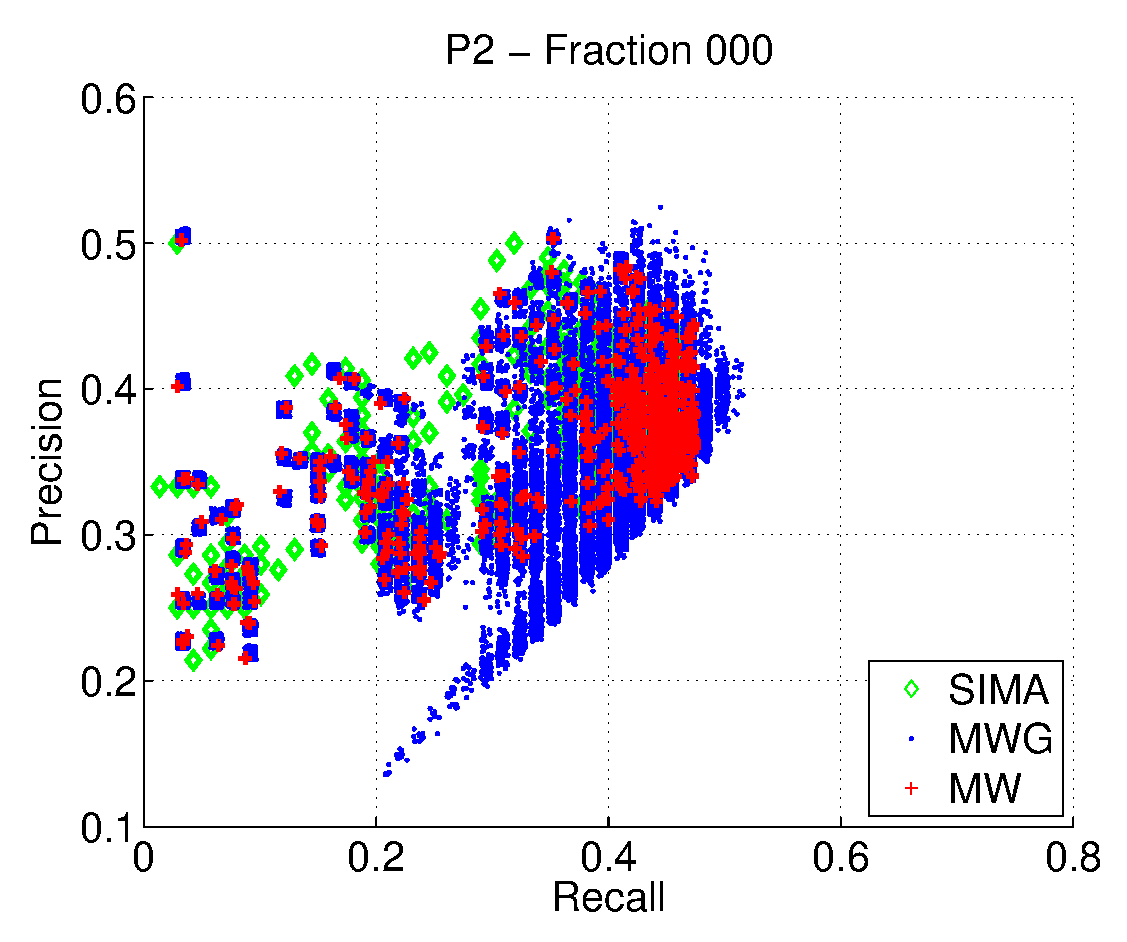
\includegraphics[scale=0.2]{04-matching/figures/figure_2c.eps}
%     \caption{P2 Fraction 000}\label{fig:figC}
%   \end{subfigure}
%   \begin{subfigure}{0.24\linewidth} \centering
%     \includegraphics[scale=0.2]{04-matching/figures/figure_2d.eps}
%     \caption{P2 Fraction 100}\label{fig:figD}
%   \end{subfigure}
%\caption{Precision and recall training performance for all parameters (m/z, RT tolerance, $\alpha$ and $g_{tol}$) varied in the experiment for the fractions containing the most (Fig. 2a \& 2c) and least (Fig. 2b \& 2d) number of features in the P1 and P2 datasets. \textbf{REDRAW IN MATPLOTLIB}} \label{fig:single-fraction-results}
%\end{figure}

\begin{figure}[!htbp]
\centering
\subfloat[P1 Fraction 000]{%
	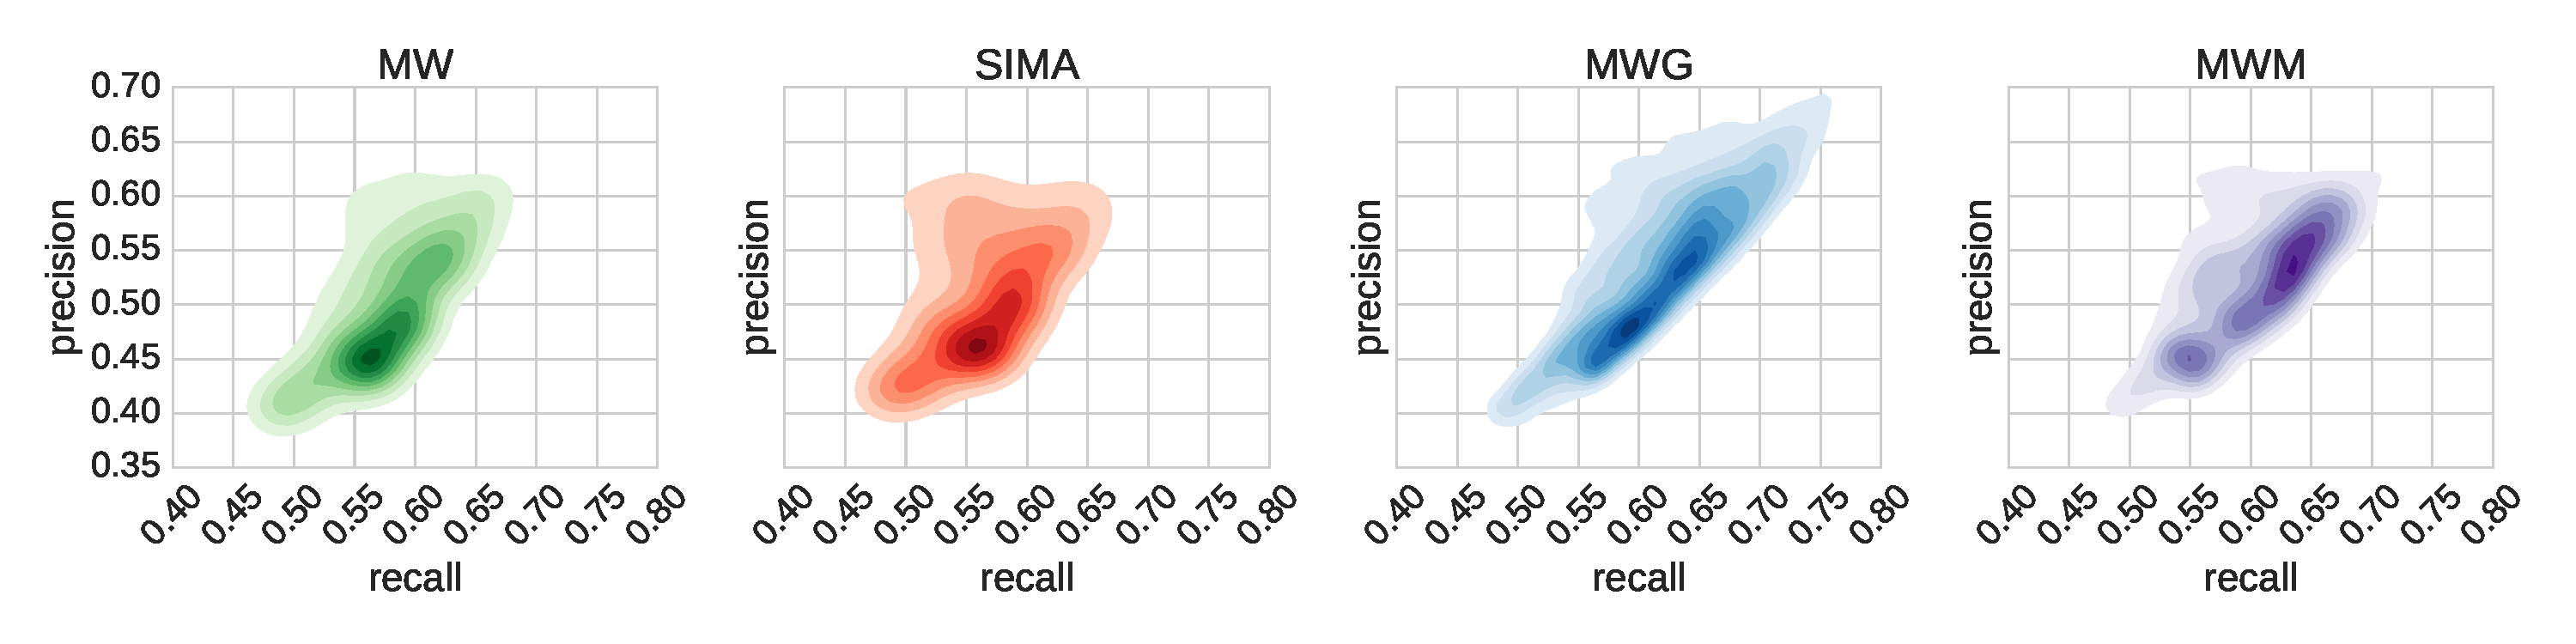
\includegraphics[clip,width=1.0\columnwidth]{04-matching/figures/P1_000_new.pdf}%
	\label{fig:figA}
}
\
\subfloat[P1 Fraction 100]{%
	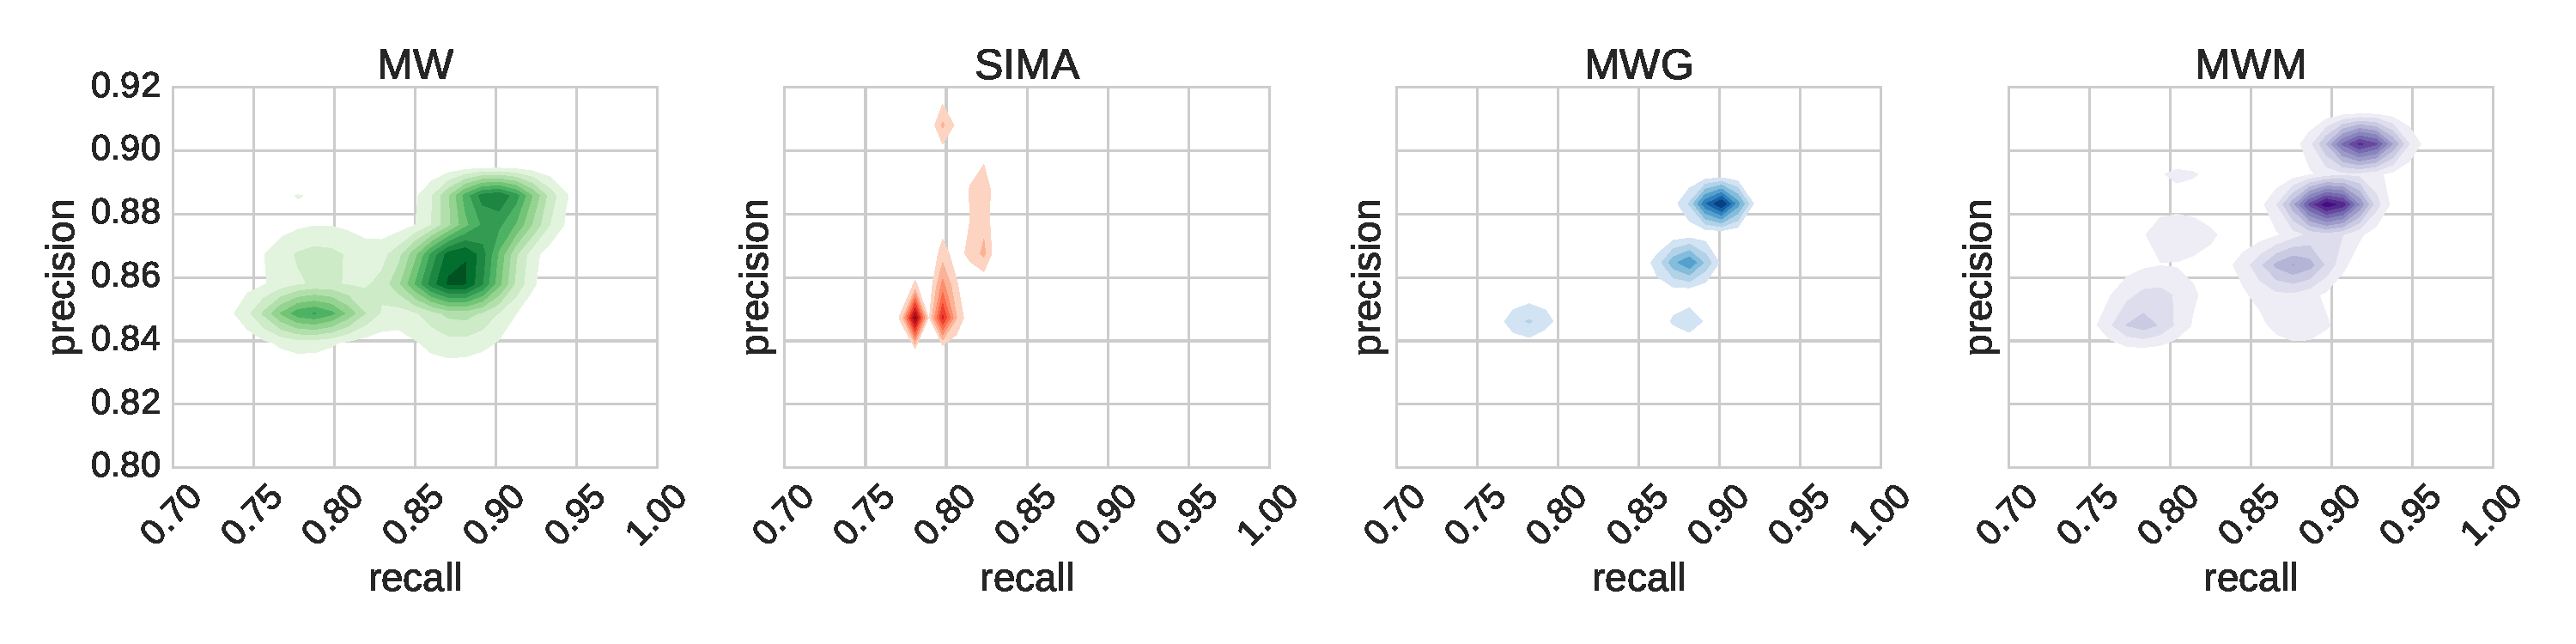
\includegraphics[clip,width=1.0\columnwidth]{04-matching/figures/P1_100_new.pdf}%
	\label{fig:figB}
}
\caption{Precision and recall training performance for all parameters (m/z, RT tolerance, $\alpha$ and $g_{tol}$) varied in the experiment for the fractions containing the most (a) and the least (b) number of features in the P1 dataset.} \label{fig:single-fraction-results-P1}
\end{figure}

\begin{figure}[!htbp]
\centering
\subfloat[P2 Fraction 000]{%
	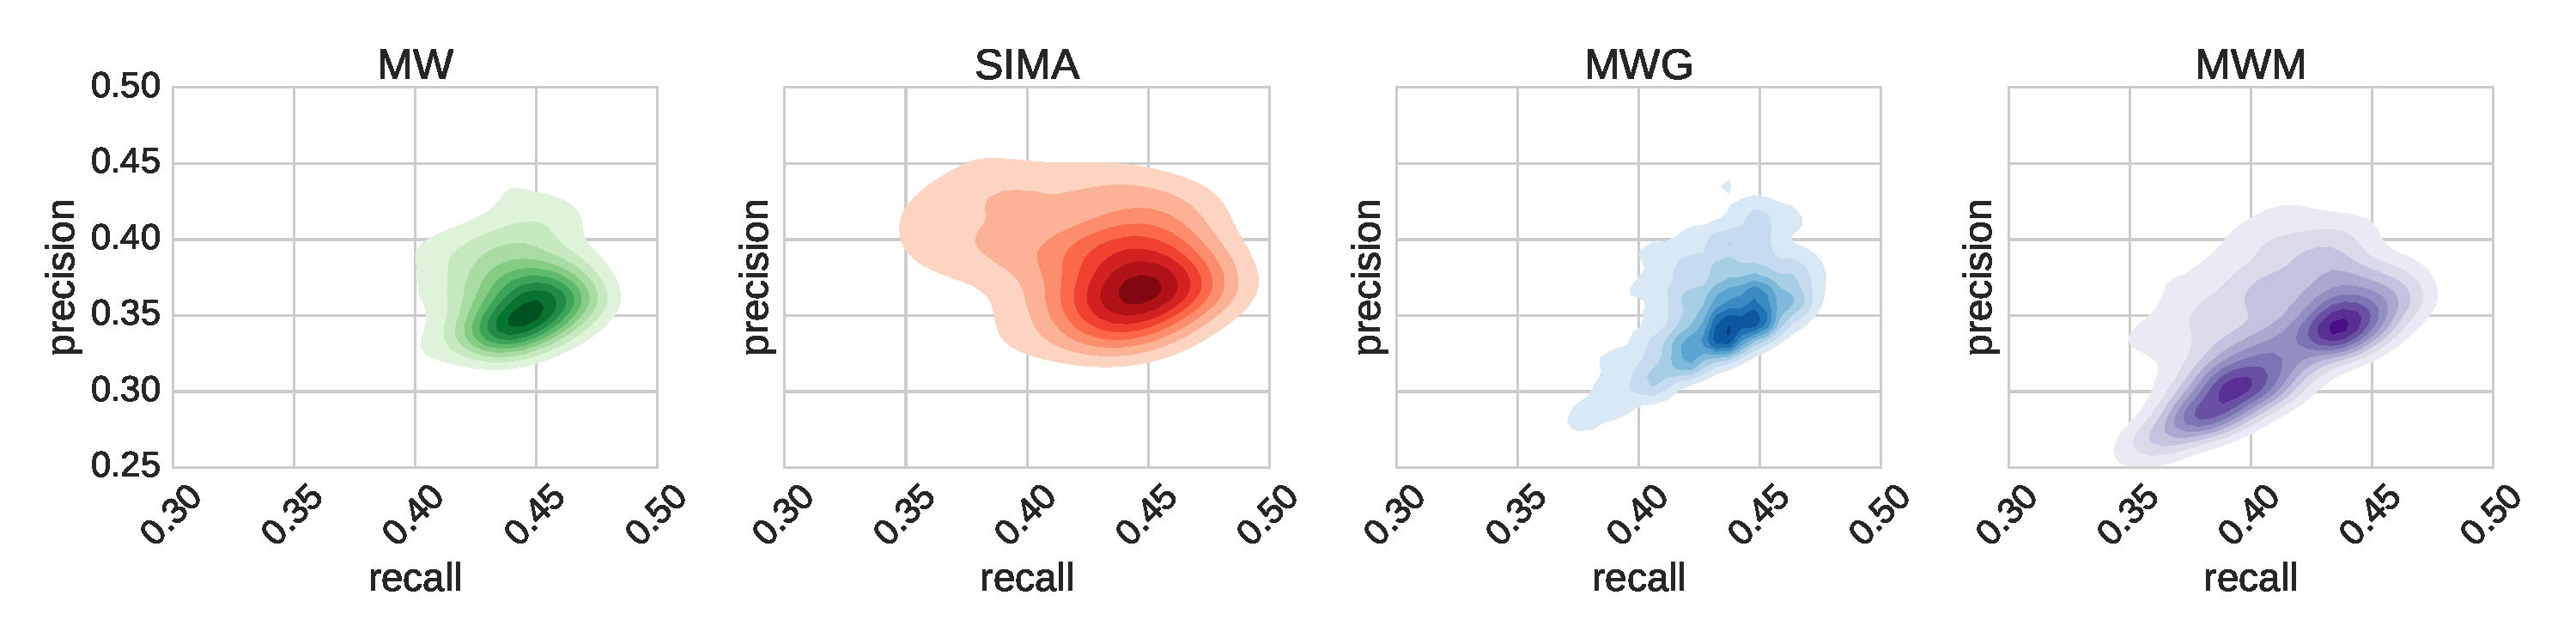
\includegraphics[clip,width=1.0\columnwidth]{04-matching/figures/P2_000_new.pdf}%
	\label{fig:figC}
}
\
\subfloat[P2 Fraction 100]{%
	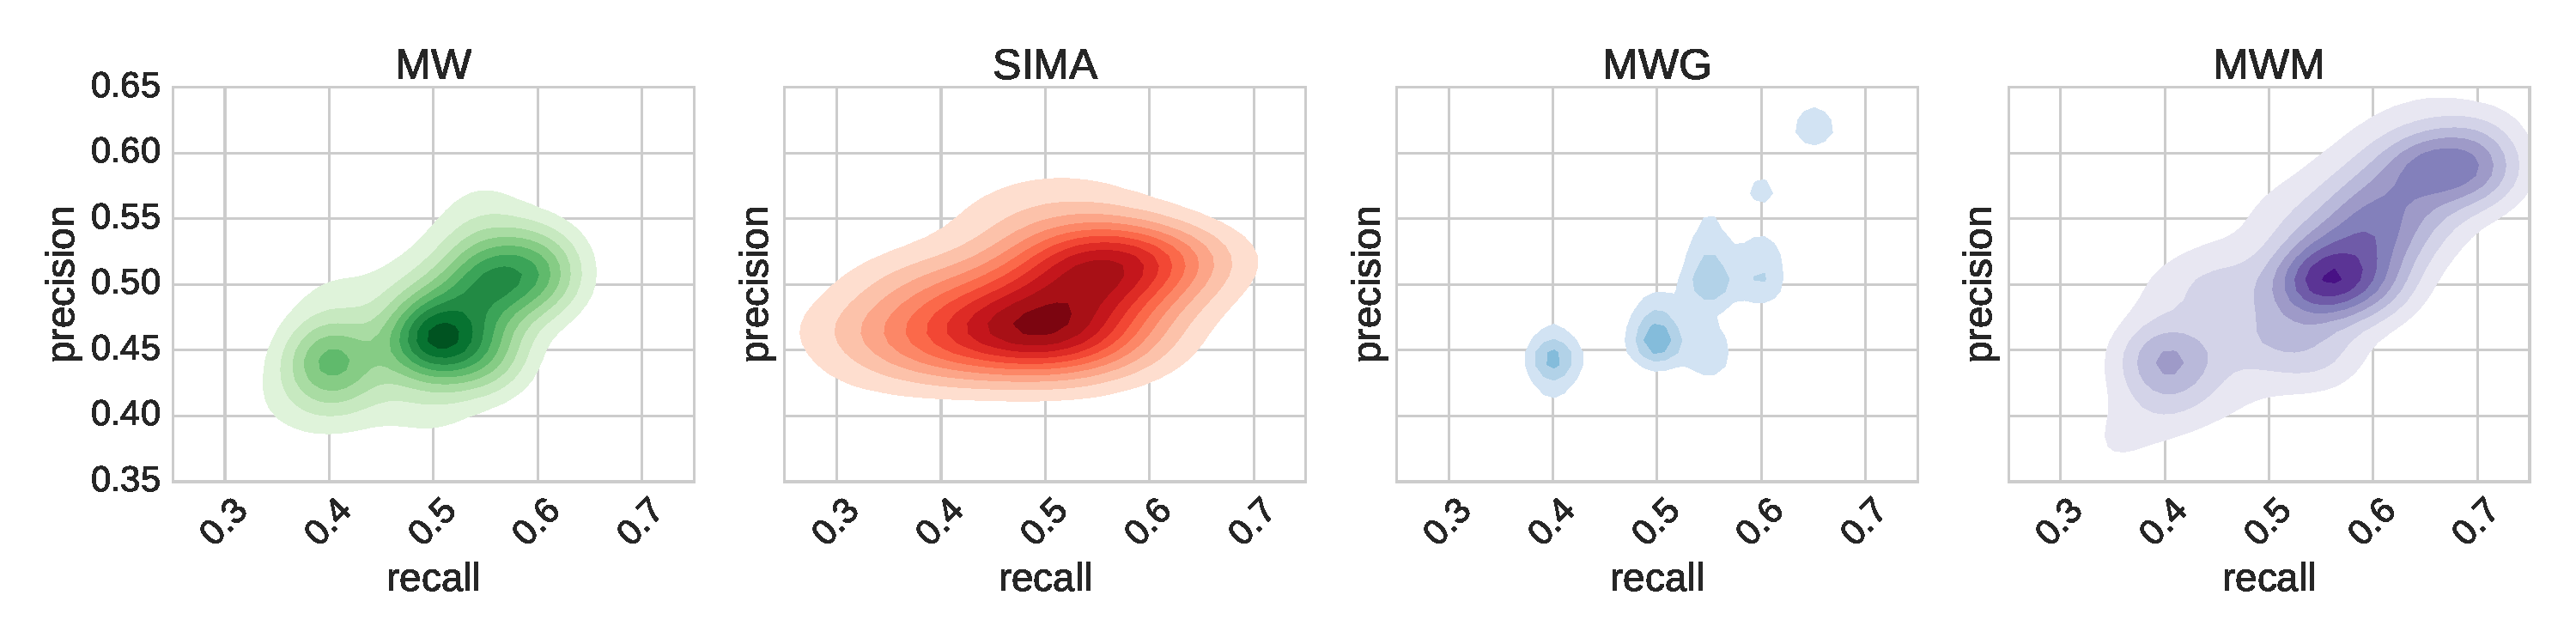
\includegraphics[clip,width=1.0\columnwidth]{04-matching/figures/P2_100_new.pdf}%
	\label{fig:figD}
}
\caption{Precision and recall training performance for all parameters (m/z, RT tolerance, $\alpha$ and $g_{tol}$) varied in the experiment for the fractions containing the most (a) and the least (b) number of features in the P2 dataset.} \label{fig:single-fraction-results-P2}
\end{figure}

\subsubsection{Multiple-fractions Experiment}

The single-fraction experiment does not represent a very realistic scenario as the optimal parameters were determined with respect to an alignment ground truth; practitioners might not possess that information in real analytical situations. In this experiment, we improved upon the single-fraction experiments by using each fraction in each dataset as the training set and the remaining fractions as the testing set. Parameters were optimised on the training set and performance evaluations were performed on the testing set. This training-testing procedure produces 6 measurements for P1 and 5 measurements for P2, corresponding to the number of training fractions in each dataset. The overall F$_1$ score reported for each measurement is the average F$_1$ scores from individual testing fractions. The aim of this experiment is to investigate how well the different methods generalise to data that may have slightly different characteristics from that used to optimise the parameters -- i.e.\ how critical the particular parameter values are.

Tables~\ref{tab:within-P1} and \ref{tab:within-P2} show the F$_{1}$ score across measurements. On P1, the best overall performance is achieved by our methods that incorporate clustering information into alignment (MWG, MWM). On P2, the results are less homogeneous, with no method consistently performing best on all the different testing fractions. In the case of the noisiest data (dataset P2 fraction 000), our proposed approach incorporating greedy clustering (MWG) shows a decrease in overall testing performance instead. This is because the greedy clustering method used is sensitive to the choice of parameters and do not generalise well across the different fractions of P2. For instance, the best MWG's grouping tolerance parameter for fraction 000 is 5 seconds, while it is 1 second for fraction 080. The results suggest the dependence of our methods on the quality of groupings of IP peaks in order to generalise well on different runs. The heterogeneous testing performance in the multiple-fractions experiment of P2 shows that no method performs best and the choice of optimal parameters that work for certain runs do not generalise well to others on datasets with very high RT variability.

\begin{table}[!htbp]
\noindent \begin{centering}
\begin{tabular}{|l|c|c|c|c|c|}
\hline 
\multirow{2}{*}{\textbf{Training Frac.}} & \multicolumn{5}{c|}{\textbf{Testing Performance}}\tabularnewline
\cline{2-6} 
 & \textbf{Join} & \textbf{SIMA} & \textbf{MW} & \textbf{MWG} & \textbf{MWM}\tabularnewline
\hline 
\hline 
\multirow{1}{*}{{000}} & {0.82} & {0.85} & {0.82} & \textbf{0.86} & \textbf{0.86}\tabularnewline
\hline 
\multirow{1}{*}{{020}} & {0.78} & {0.76} & {0.78} & \textbf{0.79} & {0.75}\tabularnewline
\hline 
\multirow{1}{*}{{040}} & {0.78} & {0.76} & {0.77} & {0.79} & \textbf{0.81}\tabularnewline
\hline 
\multirow{1}{*}{{060}} & {0.78} & {0.78} & {0.77} & \textbf{0.84} & {0.83}\tabularnewline
\hline 
\multirow{1}{*}{{080}} & {0.71} & {0.73} & {0.72} & {0.77} & \textbf{0.78}\tabularnewline
\hline 
\multirow{1}{*}{{100}} & {0.75} & {0.77} & {0.74} & {0.76} & \textbf{0.78}\tabularnewline
\hline 
\end{tabular}
\par\end{centering}
\caption[Multiple-fractions experiment results for the
P1 dataset.]{\label{tab:within-P1}Multiple-fractions experiment results for the
P1 dataset. For each training fraction, the reported testing performance is the average of individual F$_1$ scores from the testing fractions. The top-performing method (highest F$_1$ score) is highlighted in bold.}
\end{table}

\begin{table}[!htbp]
\noindent \begin{centering}
\begin{tabular}{|c|c|c|c|c|c|}
\hline 
\multirow{2}{*}{\textbf{Training Frac.}} & \multicolumn{5}{c|}{\textbf{Testing Performance}}\tabularnewline
\cline{2-6} 
 & \textbf{Join} & \textbf{SIMA} & \textbf{MW} & \textbf{MWG} & \textbf{MWM}\tabularnewline
\hline 
\hline 
\multirow{1}{*}{{000}} & {0.62} & \textbf{0.64} & {0.61} & {0.48} & {0.61}\tabularnewline
\hline 
\multirow{1}{*}{{020}} & \textbf{0.58} & {0.56} & {0.55} & {0.43} & {0.55}\tabularnewline
\hline 
\multirow{1}{*}{{040}} & {0.52} & \textbf{0.56} & \textbf{0.56} & {0.41} & \textbf{0.56}\tabularnewline
\hline 
\multirow{1}{*}{{080}} & {0.56} & {0.50} & {0.50} & {0.50} & \textbf{0.57}\tabularnewline
\hline 
\multirow{1}{*}{{100}} & \textbf{0.63} & {0.57} & {0.56} & {0.44} & {0.57}\tabularnewline
\hline 
\end{tabular}
\par\end{centering}
\caption[Multiple-fractions experiment results for the
P2 dataset.]{\label{tab:within-P2}Multiple-fractions experiment results for the
P2 dataset. For each training fraction, the reported testing performance is the average of individual F$_1$ scores from the testing fractions. The top-performing method (highest F$_1$ score) is highlighted in bold.}
\end{table}

%%%%%%%%%%%%%%%%%%%%%%%%%%%%%%%%%%%%%%%%%%%%%%%%%%%%%%%%%%%%
%%%%%%%%%%%%%%%%%%%%%%%%%%%%%%%%%%%%%%%%%%%%%%%%%%%%%%%%%%%%
%%%%%%%%%%%%%%%%%%%%%%%%%%%%%%%%%%%%%%%%%%%%%%%%%%%%%%%%%%%%
%%%%%%%%%%%%%%%%%%%%%%%%%%%%%%%%%%%%%%%%%%%%%%%%%%%%%%%%%%%%
%%%%%%%%%%%%%%%%%%%%%%%%%%%%%%%%%%%%%%%%%%%%%%%%%%%%%%%%%%%%

\subsection{Metabolomic and Glycomic Datasets}
\label{sub:Metabolomic-glycomic-experiments}

We further explore the performance of our proposed methods on the metabolomic and glycomic datasets. From the full dataset, we randomly extracted 30 pairs of runs as the training sets and another 30 pairs of runs as the testing sets. Each training set is paired to a testing set. Parameters were optimised on the training set and the best attainable performance reported as the training performance. Generalisation performance is evaluated on testing sets using the optimal parameters from the training stage.

Figures~\ref{fig:glyco-datasets-alignment-train} and \ref{fig:glyco-datasets-alignment-test} summarise the results from the experiments. We see that all methods perform better on the glycomic set than on the metabolomic set. This is explained by the fact that the metabolomic runs represent a generally more challenging alignment scenario with significantly more features to align. MW performs identically to SIMA on both datasets due to the similar form of Mahalanobis distance function used. This is despite the differences in the actual matching method that establishes feature correspondences in SIMA and MW, emphasising the fact that the actual choice of matching function might be less important than other factors, such as the determination of similarity scores between peaks. On the glycomic dataset, adding clustering information improves the training performance, with an increase in the mean of the F$_1$ scores across 30 measurements from 0.89 (MW) to 0.93 (MWG) and 0.92 (MWM). This also translates into statistically significant improvements on the testing sets for both MWG (p=0.01, paired t-test) and MWM (p=0.002, paired t-test) over MW.

On the metabolomic dataset, where it is potentially harder to produce good clustering results due to the larger number of peaks and the more complex elution profile, we observe improvements in the mean of the F$_1$ scores from 0.83 (MW) to 0.90 (MWG) and 0.85 (MWM) on the training sets. These are also statistically significant improvements for both MWG (p{\textless}0.001, paired t-test) and MWM (p{\textless}0.001, paired t-test) over MW. The training results confirm our hypothesis that indeed incorporating clustering information (by modifying the similarity matrix used for matching in the proposed manner) can be used to help improve matching results over the case when such information is not used. However, this does not translate into any statistically significant improvements on the testing sets, suggesting that for the metabolomic dataset evaluated here, our proposed methods are also sensitive to parameter choices, and the choices of particular parameters (especially for the clustering step) that work on some runs may not generalise well to others. The results shown for running MWG on the metabolomic data in Figures~\ref{fig:glyco-datasets-alignment-train} and \ref{fig:glyco-datasets-alignment-test} takes into account the Pearson correlations of the chromatographic shapes between peaks during the clustering process, since that information is available and straightforward to incorporate into the greedy clustering process. Results for MWG that consider only the RT values are presented and discussed in the following paragraph. 

\begin{figure}[!htbp]
\centering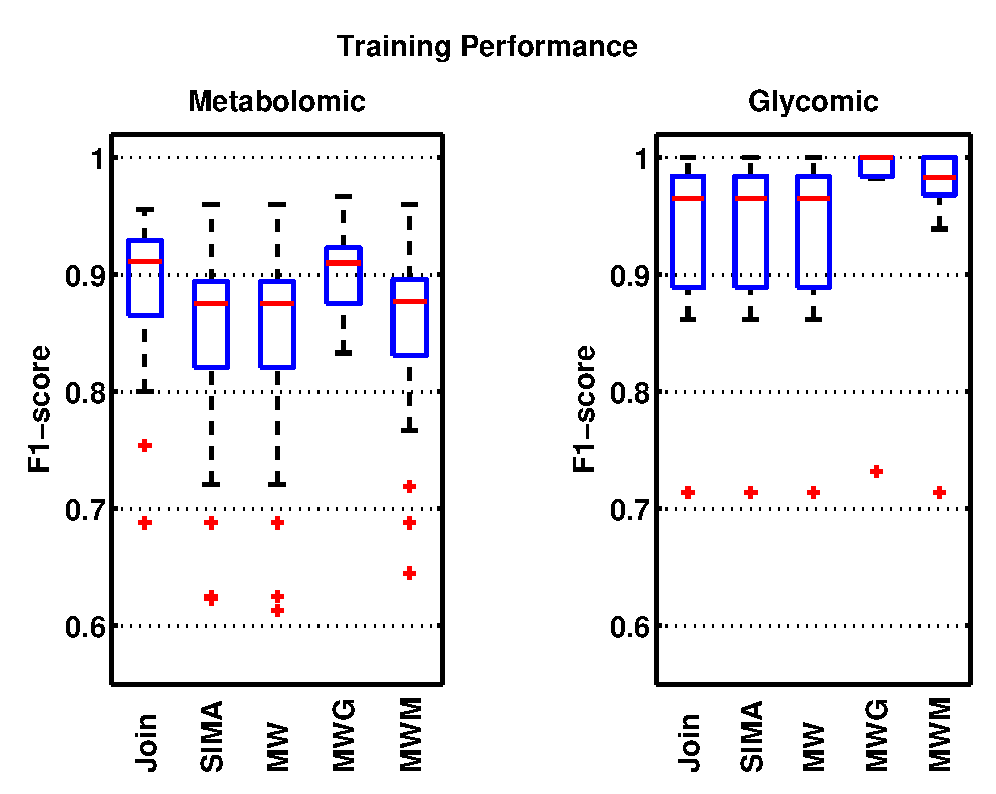
\includegraphics[width=0.65\columnwidth]{04-matching/figures/figure_3.eps}
\centering\caption{\label{fig:glyco-datasets-alignment-train}Training performance shows the best F$_1$ scores obtained by each method on 30 pairs of randomly-selected metabolomic and glycomic training sets.}
\end{figure}

\begin{figure}[!htbp]
\centering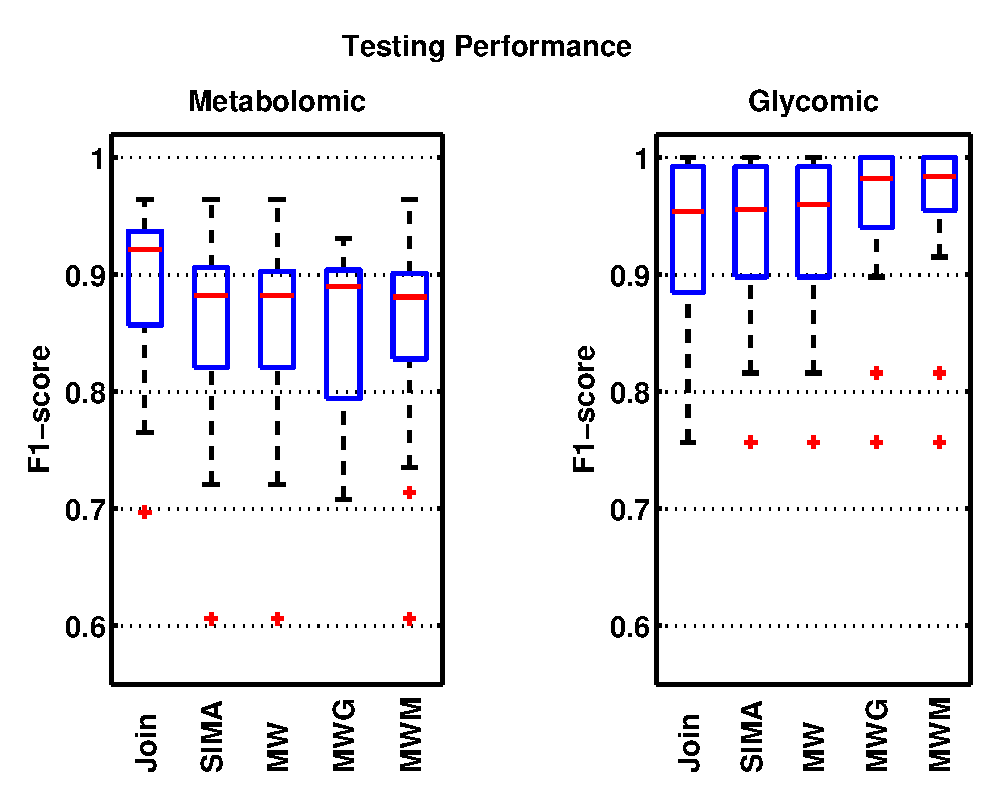
\includegraphics[width=0.65\columnwidth]{04-matching/figures/figure_4.eps}
\centering\caption{\label{fig:glyco-datasets-alignment-test}Testing performance shows how well each method generalise on the 30 different testing sets, each evaluated using the optimal training parameters from its corresponding training set.}
\end{figure}

We also compared the results for MWG on both the training and testing sets on the standard metabolomic dataset when the greedy grouping is performed using only RT information (MWG (RT)) and when chromatographic peak shape correlations are also considered (MWG(RT+PS)) during the grouping process. Statistically significant differences can be observed on the training performance of Figure \ref{fig:MWG-RT-andPS}, with the mean of $F\ensuremath{_{1}}$ scores for MW 0.83, MWG(RT) 0.88 and MWG(RT+PS) 0.90. However, this does not translate to any improvements on the testing sets, with the mean of $F\ensuremath{_{1}}$ scores for MW 0.86, MWG(RT) 0.83 and MWG(RT+PS) 0.85. Introducing clustering information when only RT information is used during the clustering process (MWG(RT)) reduces testing performance. The training results suggest that where additional information such as chromatographic peak shapes are available, they should be used for the clustering step in the proposed methods. However, the lack of any statistically significant testing improvements between MW and MWG (RT+PS), suggest that the optimal parameters from training runs do not generalise well to different testing runs for the greedy clustering approach in general, especially for complex metabolomic runs, with large number of features that tend to closely co-elute with each other.

\begin{figure}[!htbp]
\noindent \begin{centering}
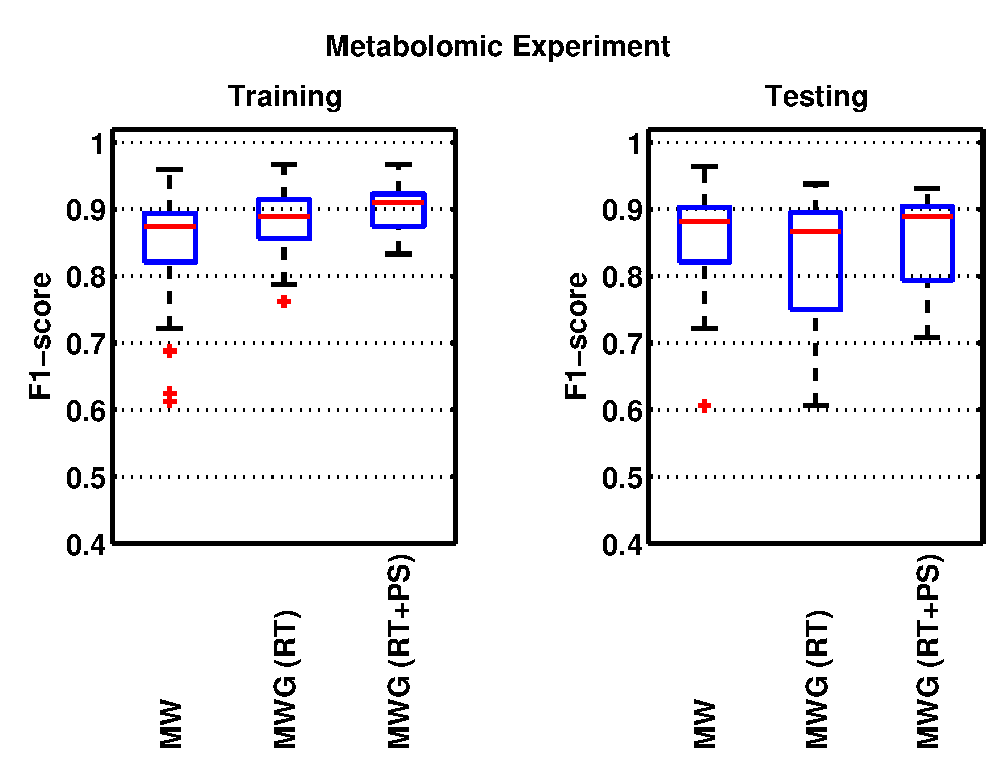
\includegraphics[width=0.6\textwidth]{04-matching/figures/supp_figure_3}
\par\end{centering}

\caption{\label{fig:MWG-RT-andPS}Comparisons in matching performance when
greedy clustering with retention time (MWG(RT)) and peak shape correlations
(MWG(RT+PS)) are used.}
\end{figure}

\subsection{Running Time}

Computational times of the proposed methods are primarily affected by the number of features in the runs being aligned and to some extent, the thresholding parameters used during similarity score computation and feature matching. Table \ref{tab:Running-Time-P1} reports the measured running time for each proposed method using the parameters that give the best training performance). For each fraction being aligned, the running times were measured three times on a standard laptop with Intel Core i5 CPU running at 2.5 GHz, and the average value reported for matching only (MW), matching incorporating greedy clustering (MWG) and matching incorporating mixture model clustering (MWM). The time complexity of the mixture-model clustering step in MWM is $O(N)$ where $N$ is the number of features in the run being clustered. We took 2000 posterior samples, discarding the first 1000 samples during the burn-in period. The number of samples were chosen to ensure convergence to the stationary distribution during inference. 

\begin{table}[!htbp]
\noindent \begin{centering}
\begin{tabular}{|c|c|c|c|c|}
\hline 
\textbf{Fraction} & \textbf{Total Features} & \textbf{MW} & \textbf{MWG} & \textbf{MWM}\tabularnewline
\hline 
\hline 
000 & 10606 & 9 & 12 & 2700\tabularnewline
\hline 
020 & 2135 & 1 & 2 & 524\tabularnewline
\hline 
040 & 2188 & 2 & 2 & 540\tabularnewline
\hline 
060 & 3342 & 2 & 3 & 825\tabularnewline
\hline 
080 & 2086 & 2 & 2 & 505\tabularnewline
\hline 
100 & 1326 & 1 & 2 & 321\tabularnewline
\hline 
\end{tabular}
\par\end{centering}
\caption{\label{tab:Running-Time-P1}Example measured execution time in seconds on fractions of the P1 dataset}
\end{table}

\section{Conclusion}

\label{sec:conc}
In this chapter, we have proposed a novel peak matching method that incorporates related peak information to improve alignment performance. The method takes related peak information in the form of peak-by-peak binary or real-valued similarity matrices and as such is independent of the particular method used to compute these. The method fits into the category of direct matching approaches --- those alignment methods that do not perform an explicit time-warping phase. Our experimental results demonstrate the potential of this approach. From the training results, we see evidence of performance improvement across all evaluated datasets by incorporating grouping information into the matching process in the proposed manner. With the exception of the metabolomic dataset, both the greedy and model-based clustering approaches evaluated in our experiments rely only on the \ac{RT} information for grouping IP peaks. By looking at the testing performance, our results also explore the ability of the evaluated methods to generalise on different runs using less than optimal parameters. This is important because in the actual analytical situation of LC-MS data, neither the optimal parameters nor the alignment ground truth is known. 

Note that our method relies on grouping of IP peaks, and this introduces additional user-defined parameters. However, as our experiments have shown, in some settings, it may be much easier to produce good groupings of IP peaks than accurately determine \ac{RT} window parameters (the same grouping parameters were used for all evaluation datasets in the case of mixture-model clustering). Depending on the nature of the data, parameters relating to within-run characteristics (e.g. \ac{RT} window for grouping IP peaks) may be more likely to generalise across runs and experiments than parameters relating to between-run characteristics (particularly \ac{RT}). For example, changes in the \ac{LC} column would likely result in related-peaks still co-eluting but could significantly change the absolute \ac{RT}. 

It would be interesting to investigate in greater detail any performance improvements that can be obtained from using other peak grouping methods, such as \cite{Rogers2012} that uses a mixture model of peak shape correlations or \cite{Daly2014} that considers the dependencies between adduct and isotopic peaks when clustering. Exploring alternative approximate matching algorithms (such as the scaling algorithm in \cite{Maximum2011}, which provides a $(1-\epsilon)$ approximation of the maximum weighted matching in optimal linear time for any $\epsilon$) and evaluating the benefits of incorporating different clustering approaches into our proposed alignment method are avenues for future work. Finally, the different alignment methods evaluated in this chapter also suffer from variable behaviours depending on the order of the runs being aligned \cite{Smith2014}. This is particularly true in the case of alignment of multiple runs (typical in large-scale LC-MS studies), where the final alignment results are often constructed through merging of intermediate alignments of pairwise runs. Different alignment methods may employ a different merging approach, for example, Join merges the intermediate results towards a reference run while SIMA allows the possibility of using a greedy hierarchical merging scheme. Systematic evaluation on how the chosen merging scheme may influence alignment performance is beyond the scope of this chapter and is an item for future work.

A limitation of the proposed approaches lies in the fact that the clustering of IP peaks are performed based on RT only. The valuable information present in the m/z domain is not used for clustering. The grouping of IP peaks based on their m/z information is less straightforward as peaks that are related (sharing close RT values) do not necessarily have m/z values that are close to each other. In the evaluation on the complex metabolomic dataset, we observe that the proposed approach using RT clustering manages to improve training performance (due to overfitting) but fails to produce any statistically significant improvement in the testing performance due to its limited generalisation ability. In the next chapter, we address this issue by focusing specifically on metabolomics and proposing a clustering model that explicitly takes into account the chemical relationship between IP peaks in LC-MS-based metabolomics. 